\documentclass[
  12pt,
  oneside,
  a4paper,
  english,
  brazilian
  ]{abntex2}

% ---
% Pacotes básicos
% ---
\usepackage[scaled]{helvet}
\renewcommand{\familydefault}{\sfdefault}
\usepackage[T1]{fontenc}
\usepackage[utf8]{inputenc}
\usepackage{indentfirst}
\usepackage{color}
\usepackage{graphicx}
\usepackage{microtype}
\usepackage{lipsum}
\usepackage{amsthm}
\usepackage{url}
\usepackage{float}
\setlength{\marginparwidth}{2cm}
\usepackage{todonotes}
\usepackage{tikz}
\usetikzlibrary{arrows.meta, positioning}
\usepackage{amsmath, amssymb}
\usepackage{enumitem}

% ---
% Configurações do hyperref
% ---
\hypersetup{
    colorlinks=true,
    linkcolor=black,
    citecolor=black,
    urlcolor=black,
    filecolor=black
}

% ---
% Ajustes de fonte para títulos
% ---
\renewcommand{\ABNTEXchapterfont}{\sffamily\bfseries}
\renewcommand{\ABNTEXchapterfontsize}{\LARGE}
\renewcommand{\ABNTEXsectionfont}{\sffamily\bfseries}
\renewcommand{\ABNTEXsectionfontsize}{\Large}
\renewcommand{\ABNTEXsubsectionfont}{\sffamily\bfseries}
\renewcommand{\ABNTEXsubsectionfontsize}{\large}

\renewcommand{\thepage}{\arabic{page}}
\renewcommand{\thechapter}{\arabic{chapter}}
\renewcommand{\thesection}{\thechapter.\arabic{section}}
\renewcommand{\thesubsection}{\thesection.\arabic{subsection}}
\renewcommand{\thesubsubsection}{\thesubsection.\arabic{subsubsection}}
\renewcommand{\thefigure}{\arabic{figure}}
\renewcommand{\thetable}{\arabic{table}}

\captionstyle{\sffamily\bfseries}
\captionnamefont{\sffamily\bfseries}
\captiontitlefont{\sffamily}

% ---
% Ambientes de teorema
% ---
\theoremstyle{definition}
\newtheorem{definicao}{Definição}[chapter]
\newtheorem{teorema}[definicao]{Teorema}
\newtheorem{lema}[definicao]{Lema}
\newtheorem{exemplo}[definicao]{Exemplo}
\newtheorem{propriedade}[definicao]{Propriedade}

% ---
% Proteção para Metadados do PDF
% ---
\pdfstringdefDisableCommands{%
  \def\\{ }%
  \def\par{ }%
  \def\vspace#1{ }%
  \def\sffamily{}%
  \def\bfseries{}%
}

% ---
% Arquivo de Bibliografia Embutido
% ---
\begin{filecontents*}{referencias.bib}

@book{boaventura2009,
  author    = {Boaventura, Oswaldo and Jurkiewicz, Samuel},
  title     = {Grafos},
  publisher = {Editora Blucher},
  year      = {2009}
}

@misc{silva2020,
  author = {Da Silva, Luiz Fernando},
  title  = {Uma Proposta de Sequência Didática para o Ensino Médio:
            Introdução ao Estudo da Teoria dos Grafos com GeoGebra},
  year   = {2020},
  note   = {6 mai. 2020}
}

@book{cormen2009,
  author    = {Cormen, T. H. and Leiserson, C. E. and Rivest, R. L. and Stein, C.},
  title     = {Introduction to Algorithms},
  edition   = {3},
  publisher = {MIT Press},
  address   = {Cambridge, Mass.},
  year      = {2009}
}

@manual{brasil2002,
  organization = {Brasil},
  title        = {{PCN+} Ensino Médio: Orientações Educacionais Complementares
                  aos Parâmetros Curriculares Nacionais -- Ciências da Natureza,
                  Matemática e suas Tecnologias},
  address      = {Brasília},
  publisher    = {MEC/SEMTEC},
  year         = {2002}
}

@misc{jurkiewicz2007,
  author = {Jurkiewicz, S.},
  title  = {Grafos: Uma introdução},
  year   = {2007},
  note   = {Programa de Iniciação Científica da OBMEP 2007}
}

@mastersthesis{malta2008,
  author  = {Malta, G. H. S.},
  title   = {Grafos no ensino médio: uma inserção possível},
  school  = {Universidade Federal do Rio Grande do Sul},
  address = {Porto Alegre},
  year    = {2008}
}

@article{rodrigues2021,
  author  = {Rodrigues, A. B. and Silva, C. D.},
  title   = {O ensino de grafos e a cultura digital: novas perspectivas
             para a matemática escolar},
  journal = {Revista de Educação Matemática},
  volume  = {10},
  number  = {2},
  pages   = {1--15},
  year    = {2021}
}

@book{diestel2017,
  author    = {Diestel, Reinhard},
  title     = {Graph Theory},
  edition   = {5},
  publisher = {Springer},
  address   = {Berlin},
  year      = {2017}
}

@book{wilson1996,
  author    = {Wilson, Robin J.},
  title     = {Introduction to Graph Theory},
  edition   = {4},
  publisher = {Longman},
  address   = {London},
  year      = {1996}
}

@book{bondy1976,
  author    = {Bondy, J. A. and Murty, U. S. R.},
  title     = {Graph Theory with Applications},
  publisher = {North-Holland},
  address   = {New York},
  year      = {1976}
}

@book{rosen2012,
  author    = {Rosen, Kenneth H.},
  title     = {Discrete Mathematics and Its Applications},
  edition   = {7},
  publisher = {McGraw-Hill},
  address   = {New York},
  year      = {2012}
}

@article{euler1736,
  author  = {Euler, Leonhard},
  title   = {Solutio problematis ad geometriam situs pertinentis},
  journal = {Commentarii Academiae Scientiarum Imperialis Petropolitanae},
  volume  = {8},
  pages   = {128--140},
  year    = {1741},
  note    = {Apresentado em 1736}
}

@misc{brasil1996,
  author   = {Brasil},
  title    = {Lei n\textordmasculine{} 9.394, de 20 de dezembro de 1996:
              Estabelece as diretrizes e bases da educação nacional},
  address  = {Brasília},
  year     = {1996},
  note     = {Diário Oficial da União, Brasília, DF, 23 dez. 1996.
              Disponível em: \url{http://www.planalto.gov.br/ccivil_03/leis/l9394.htm}. Acesso em: 10 jan. 2026}
}

@manual{brasil2018,
  organization = {Brasil},
  title        = {Base Nacional Comum Curricular},
  address      = {Brasília},
  publisher    = {MEC},
  year         = {2018}
}

@article{cameron1999,
  author  = {Cameron, Kathie and Edmonds, Jack},
  title   = {Some graphic uses of an even number of odd nodes},
  journal = {Annales de l'Institut Fourier},
  volume  = {49},
  number  = {3},
  pages   = {815--827},
  year    = {1999},
  doi     = {10.5802/aif.1694}
}

@article{papadimitriou1994,
  author  = {Papadimitriou, Christos H.},
  title   = {On the complexity of the parity argument and other inefficient proofs of existence},
  journal = {Journal of Computer and System Sciences},
  volume  = {48},
  number  = {3},
  pages   = {498--532},
  year    = {1994},
  doi     = {10.1016/S0022-0000(05)80063-7}
}

@incollection{thomason1978,
  author    = {Thomason, A. G.},
  title     = {Hamiltonian cycles and uniquely edge colourable graphs},
  booktitle = {Advances in Graph Theory (Cambridge Combinatorial Conf., Trinity College, Cambridge, 1977)},
  series    = {Annals of Discrete Mathematics},
  volume    = {3},
  pages     = {259--268},
  year      = {1978},
  doi       = {10.1016/S0167-5060(08)70511-9}
}

@book{polya2006,
  author    = {Polya, George},
  title     = {A arte de resolver problemas: um novo aspecto do m{\'e}todo matem{\'a}tico},
  translator= {Heitor Lisboa de Ara{\'u}jo},
  publisher = {Interci{\^e}ncia},
  address   = {Rio de Janeiro},
  year      = {2006},
  edition   = {2}
}

@manual{bahia2019,
  organization = {Bahia},
  title        = {Documento Curricular Referencial da Bahia para a Educa{\c{c}}{\~a}o Infantil e Ensino Fundamental},
  address      = {Salvador},
  publisher    = {Secretaria da Educa{\c{c}}{\~a}o do Estado da Bahia (SEC-BA)},
  year         = {2019},
  url          = {https://escolas.educacao.ba.gov.br/documento-curricular-referencial-da-bahia},
  urldate      = {2026-07-13}
}

@article{lima2022,
  author  = {Lima, P. R. and Santos, M. A.},
  title   = {A Teoria dos Grafos como ferramenta para o desenvolvimento do pensamento computacional no Ensino M{\'e}dio},
  journal = {Bolema: Boletim de Educa{\c{c}}{\~a}o Matem{\'a}tica},
  volume  = {36},
  number  = {73},
  pages   = {850--872},
  year    = {2022},
  doi     = {10.1590/1980-4415v36n73a18}
}

\end{filecontents*}

% ---
% Configuração da Bibliografia (biblatex para norma ABNT)
% ---
\usepackage{csquotes} 
\usepackage[style=abnt, hyperref=true, backend=biber]{biblatex}
\addbibresource{referencias.bib}

% ---
% Informações de dados para CAPA e FOLHA DE ROSTO
% ---
\titulo{PROPOSTA DE INSERÇÃO DO ENSINO DE GRAFOS PARA ALUNOS DO ENSINO MÉDIO DA REDE PÚBLICA}
\autor{JOSÉ GUILHERME DANTAS SILVA}
\local{Ilhéus-BA}
\data{2026}
\orientador{Prof. Dr. Romenique da Rocha Silva}
\coorientador[Coorientadora:]{Prof\textsuperscript{a}. Ma. Sara Meira Moutta}
\instituicao{%
  UNIVERSIDADE ESTADUAL DE SANTA CRUZ
  \par
  Departamento de Ciências Exatas
  \par
  Licenciatura em Matemática}
\tipotrabalho{Trabalho de Conclusão de Curso}
\preambulo{Trabalho de Conclusão de Curso apresentado ao curso de Licenciatura em Matemática, Departamento de Ciências Exatas, da UNIVERSIDADE ESTADUAL DE SANTA CRUZ, como requisito parcial para a obtenção do grau de Licenciado em Matemática.}

% ---
% Redefinição da Capa
% ---
\renewcommand{\imprimircapa}{%
  \begin{capa}%
    \centering
    
\includegraphics[width=3.5cm]{Brasão-UESC---png1.png}\\[0.4cm] 
    {\ABNTEXchapterfont\large\imprimirinstituicao}

    \vspace{2.5cm}

    {\ABNTEXchapterfont\large\imprimirautor}

    \vspace*{\fill}

    {\ABNTEXchapterfont\bfseries\LARGE\imprimirtitulo}

    \vspace*{\fill}

    {\large\imprimirlocal}\\[0.3cm]
    {\large\imprimirdata}\\[1cm]
  \end{capa}
}

% ---
% Configurações de aparência do PDF final
% ---
\hypersetup{
    pdftitle  = {\imprimirtitulo},
    pdfauthor = {\imprimirautor}
}

\setlength{\parindent}{1.25cm}
\setlength{\parskip}{0.2cm}

% ============================================================
% INÍCIO DO DOCUMENTO
% ============================================================
\begin{document}
\selectlanguage{brazilian}
\frenchspacing

% ----------------------------------------------------------
% ELEMENTOS PRÉ-TEXTUAIS
% ----------------------------------------------------------
\pretextual

\imprimircapa
\imprimirfolhaderosto*

% ---
% Folha de aprovação
% ---
\begin{folhadeaprovacao}
  \begin{center}
    {\ABNTEXchapterfont\large\imprimirautor}
    \vspace*{\fill}\vspace*{\fill}
    \begin{center}
      \ABNTEXchapterfont\bfseries\Large\imprimirtitulo
    \end{center}
    \vspace*{\fill}
    \hspace{.45\textwidth}
    \begin{minipage}{.5\textwidth}
        \imprimirpreambulo
    \end{minipage}%
  
    \vspace*{\fill}
  \end{center}

  Aprovado em: Ilhéus, \_\_ de \_\_\_\_\_\_\_\_\_\_\_\_ de \_\_\_\_.
 \begin{center}
    \vspace*{0.5cm}
    \textbf{BANCA EXAMINADORA} \\
    \vspace*{1.5cm}
    \hrulefill \\
    \textbf{\imprimirorientador} (Orientador) \\
    Universidade Estadual de Santa Cruz \\
    \vspace*{1.5cm}
    \hrulefill \\
    \textbf{\imprimircoorientador} (Coorientadora) \\
    Universidade Estadual de Santa Cruz \\
    \vspace*{1.5cm}
    \hrulefill \\
    \textbf{Prof\textsuperscript{a}. Dr\textsuperscript{a}.\ Jurema Lindote Botelho Peixoto} (Examinadora) \\
    Universidade Estadual de Santa Cruz \\
  \end{center}
\end{folhadeaprovacao}

% ---
% Dedicatória
% ---
\begin{dedicatoria}
   \vspace*{\fill}
   \centering
   \noindent
   \textit{Dedico este trabalho in memoriam a meu pai, Geraldo Bezerra da Silva,
           como homenagem à sua vida e legado.}
   \vspace*{\fill}
\end{dedicatoria}

% Agradecimentos
% ---
\begin{agradecimentos} 

Agradeço a Deus, cuja bondade e misericórdia me sustentaram ao longo desta jornada.

À Universidade Estadual de Santa Cruz (UESC), instituição que me proporcionou crescimento intelectual e pessoal. Tenho a certeza de que retornarei para cursar o mestrado em Modelagem Computacional e, futuramente, contribuir como docente.

Ao meu orientador, Prof. Dr. Romenique da Rocha Silva, que aceitou me orientar sem hesitar e topou embarcar comigo neste final de jornada. Agradeço pela confiança, pela paciência e por toda a dedicação ao longo deste trabalho.

À minha coorientadora, Prof\textsuperscript{a}. Ma. Sara Meira Moutta, que acreditou em mim desde o início, quando participei da publicação do artigo com ela no ano passado. Foi graças à sua confiança e à sua área de pesquisa que meus olhos se abriram para a Teoria dos Grafos, e é por seu incentivo que pretendo seguir esta linha de pesquisa. Muito obrigado por todo o apoio incondicional.

À Prof\textsuperscript{a}. Dr\textsuperscript{a}. Jurema Lindote Botelho Peixoto, que acreditou e confiou em mim desde o início da graduação e prontamente aceitou participar da minha banca. Minha gratidão eterna.

À minha família, em especial à minha mãe, Edileusa Gualberto Dantas (Inha), e à minha avó, Doraci Maria da Silva (Vó Peró), pelo amor incondicional; às minhas irmãs, Victória Regina (Vick) e Claudineia (Lela), que nunca deixaram de acreditar em mim, mesmo quando eu duvidava de mim mesmo. Aos meus animais de estimação, em especial ao meu gato Bimbo, que foi meu fiel parceiro nas noites em claro, compartilhando angústias e fórmulas espalhadas em papéis.

Aos meus amigos e colegas, em especial Juan Cerqueira (Calopsita), meu parceiro de graduação que se tornou um irmão; Tarcísio Miguel (Sapo Cego), Natália Oliveira (Choquito) e André (Android), cujo apoio, companheirismo e cumplicidade foram essenciais para que eu não desistisse.

Ao meu professor do ensino médio, Ms. Edmilson Chaves, que despertou em mim, ainda na educação básica, o desejo de seguir a carreira docente e foi fundamental na minha formação. Agradeço também aos meus supervisores de estágio e PIBID — Prof. Wellingthon Fraga, Prof\textsuperscript{a}. Luana Cerqueira e Prof\textsuperscript{a}. Daniella Feitosa — por todos os ensinamentos docentes e pela oportunidade de vivenciar a sala de aula.

A todos os alunos que passaram por mim: vocês foram fundamentais para que eu continuasse. Em muitos momentos pensei em desistir, mas vocês me mostraram a beleza da docência e me deram forças para seguir.

\end{agradecimentos}
% ---
% Epígrafe
% ---
\begin{epigrafe}
    \vspace*{\fill}
  \begin{flushright}
    \textit{``A vida é como a matemática, criamos raízes \\
    que o mundo tenta subtrair de nós, porém o que é somado \\
    de bom nos ajudará a ter a solução exata do que precisamos.''\\
    (Ester Menezes)}
  \end{flushright}
\end{epigrafe}

% ---
% Resumos
% ---
\begin{resumo}
 Este trabalho apresenta uma proposta teórica e metodológica para a inserção da Teoria dos Grafos no currículo de Matemática do Ensino Médio das escolas públicas. Diante da necessidade de alinhar o ensino às demandas da sociedade contemporânea e às diretrizes da Base Nacional Comum Curricular (BNCC), a pesquisa investiga como os conceitos de grafos podem fomentar o pensamento computacional através de uma abordagem ``desplugada'', isto é, sem a dependência de laboratórios de informática. A metodologia adotada constitui-se de uma pesquisa qualitativa de cunho bibliográfico e documental. O estudo culmina na elaboração de três propostas didáticas estruturadas sob a perspectiva da Metodologia de Resolução de Problemas, englobando a modelagem de rotas urbanas, a análise de redes sociais e o Problema do Caixeiro Viajante. Discutem-se ainda os desafios da transposição didática no cenário da escola pública, destacando o papel fundamental de programas de iniciação à docência (como o PIBID) para a exequibilidade de metodologias ativas. Conclui-se que a Matemática Discreta atua como uma ferramenta poderosa para a modelagem de fenômenos reais, tornando o aprendizado mais significativo e conectado à cultura digital.
 \vspace{\onelineskip}
 \noindent \\
 \textbf{Palavras-chave}: Teoria dos Grafos. Ensino Médio. Matemática. BNCC. Pensamento Computacional.
 \end{resumo}

\begin{resumo}[Abstract]
 \begin{otherlanguage*}{english}
   This work presents a theoretical and methodological proposal for introducing Graph Theory into the high school Mathematics curriculum of public schools. Given the need to align teaching with the demands of contemporary society and the guidelines of the National Common Curricular Base (BNCC), the research investigates how graph concepts can foster computational thinking through an ``unplugged'' approach, that is, without relying on computer labs. The adopted methodology consists of qualitative bibliographic and documentary research. The study culminates in the development of three didactic proposals structured from the perspective of Problem-Solving Methodology, encompassing the modeling of urban routes, the analysis of social networks, and the Traveling Salesperson Problem. It also discusses the challenges of didactic transposition in the public school setting, highlighting the fundamental role of teaching initiation programs (such as PIBID) for the feasibility of active methodologies. It concludes that Discrete Mathematics acts as a powerful tool for modeling real phenomena, making learning more meaningful and connected to digital culture.
 \vspace{\onelineskip}
   \noindent \\
   \textbf{Keywords}: Graph Theory. High School. Mathematics. BNCC. Computational Thinking.
 \end{otherlanguage*}
\end{resumo}

% ---
% Lista de Figuras
% ---
\pdfbookmark[0]{\listfigurename}{lof}
\listoffigures*
\cleardoublepage

\begin{siglas}
  \item[BNCC] Base Nacional Comum Curricular
  \item[LDB]  Lei de Diretrizes e Bases da Educação Nacional
  \item[PIBID] Programa Institucional de Bolsa de Iniciação à Docência
  \item[UESC] Universidade Estadual de Santa Cruz
\end{siglas}

\begin{simbolos}
  \item[$\mathcal{G}$] Grafo
  \item[$\mathcal{V}$] Conjunto de vértices de um grafo
  \item[$\mathcal{A}$] Conjunto de arestas de um grafo
  \item[$\mathcal{H}$] Subgrafo
  \item[$\delta(v)$] Grau do vértice $v$
  \item[$K_n$] Grafo completo com $n$ vértices
  \item[$|\mathcal{A}|$] Cardinalidade do conjunto de arestas (número de arestas)
  \item[$|\mathcal{V}|$] Cardinalidade do conjunto de vértices (número de vértices)
  \item[$\in$] Pertence a
  \item[$\subseteq$] Está contido em (relação de subconjunto)
  \item[$\sum$] Somatório
  \item[$\implies$] Implica (então)
  \item[$(u,\, v)$] Arco (aresta orientada) que parte de $u$ e chega em $v$
  \item[$\to$] Indica o sentido de um arco em um dígrafo
  \item[$\checkmark$] Verificação/confirmação de um resultado
\end{simbolos}

\pdfbookmark[0]{\contentsname}{toc}
\tableofcontents*
\cleardoublepage

% ----------------------------------------------------------
% ELEMENTOS TEXTUAIS
% ----------------------------------------------------------
\textual

% ==========================================================
\chapter{INTRODUÇÃO}
% ==========================================================

A contextualização do ensino da Matemática na Educação Básica, particularmente
no Ensino Médio, demanda uma constante atualização curricular que dialogue com a
complexidade e a interconectividade do mundo contemporâneo. Nesse cenário, a
Teoria dos Grafos destaca-se não apenas como um ramo fundamental da Matemática
Discreta, mas como uma ferramenta indispensável para a modelagem e a compreensão
de fenômenos reais.

A relevância desse campo transcende a abstração teórica, manifestando-se
diretamente em estruturas que definem a sociedade atual, tais como a arquitetura
de redes sociais, o planejamento eficiente de sistemas de transporte e logística,
o funcionamento de algoritmos de busca e a análise de grandes volumes de dados
(\textit{Big Data}). Compreender grafos é, portanto, compreender a linguagem
estrutural por trás dos problemas de otimização e conectividade que permeiam o
cotidiano.

Para além de sua onipresença tecnológica, o estudo de grafos apresenta uma vasta
aplicabilidade prática em áreas estratégicas do conhecimento, servindo como base
para avanços na Ciência da Computação, Engenharia, Biologia (na análise de redes
metabólicas e genéticas) e Economia. Do ponto de vista pedagógico, a introdução
desses conceitos no ambiente escolar contribui significativamente para o
desenvolvimento de competências cognitivas fundamentais. O trabalho com vértices
e arestas estimula o pensamento relacional e a capacidade de abstração,
ferramentas essenciais para a modelagem matemática, a resolução de problemas não
lineares e a interpretação de estruturas complexas.

A pertinência dessa abordagem é amplamente discutida na literatura acadêmica
atual. \textcite{rodrigues2021}, por exemplo, analisam como a inserção de
tópicos de Teoria dos Grafos pode favorecer uma formação matemática mais robusta
e conectada ao universo digital, alinhando o currículo escolar às demandas da
contemporaneidade. Sob essa ótica, defende-se que a transposição didática desse
conteúdo para o Ensino Médio é uma possibilidade real e metodologicamente
fundamentada.

A Teoria dos Grafos, área da Matemática Discreta, dedica-se ao estudo dessas
estruturas formadas por vértices e arestas, possibilitando a representação e a
análise de relações e interações em diferentes contextos. Sua presença é
identificada em diversos campos, como sistemas de transporte público, redes
sociais, circuitos elétricos, algoritmos de busca na internet, logística
empresarial e até em áreas das ciências biológicas, como no estudo das cadeias
alimentares.

Apesar da ampla aplicabilidade, a Teoria dos Grafos ainda não recebe a devida
atenção no Ensino Médio da rede pública, cujos currículos e livros didáticos
priorizam conteúdos considerados clássicos da Matemática, muitas vezes
desvinculados das demandas tecnológicas e sociais contemporâneas. Essa lacuna
dificulta que os estudantes compreendam o potencial da Matemática para analisar e
propor soluções para problemas atuais.

No contexto do Novo Ensino Médio e da Base Nacional Comum Curricular (BNCC), que
enfatizam a contextualização, a interdisciplinaridade e o desenvolvimento do
pensamento computacional, a ausência da Teoria dos Grafos mostra-se ainda mais
significativa. Nesse sentido, a questão central que orienta este trabalho consiste
em investigar de que maneira é possível propor a inserção teórica da Teoria dos
Grafos no Ensino Médio da rede pública, de forma contextualizada, interdisciplinar
e em consonância com as diretrizes da BNCC.

Para dar conta dessa questão, o presente trabalho está organizado em capítulos
que se articulam entre si. O Capítulo~\ref{cap:fundamentos} apresenta os
fundamentos teóricos da Teoria dos Grafos e o estado da arte sobre seu ensino.
O Capítulo~\ref{cap:bncc} realiza uma análise documental da BNCC, identificando
as conexões entre a Teoria dos Grafos e as competências e habilidades previstas
para o Ensino Médio. O Capítulo~\ref{cap:proposta}, por fim, apresenta a proposta
didática propriamente dita, articulando os conceitos teóricos e as atividades
sugeridas com as diretrizes curriculares e as estratégias pedagógicas
recomendadas pela literatura.

\section{Objetivo Geral}

Elaborar uma abordagem teórica para a inserção da Teoria dos Grafos na Matemática
do Ensino Médio da rede pública de ensino, destacando possibilidades de
contextualização, interdisciplinaridade e inovação curricular no ensino da
Matemática.

\section{Objetivos Específicos}

\begin{itemize}
  \item Investigar a relevância da Teoria dos Grafos no contexto da Educação do
        Ensino Médio e sua relação com as competências e habilidades previstas na
        BNCC;
 \item Identificar exemplos de aplicações de grafos em situações do cotidiano e
        de outras áreas do conhecimento, capazes de tornar o aprendizado mais
        significativo para os estudantes;
 \item Pesquisar potenciais estratégias didáticas para a introdução dos conceitos
        de grafos no Ensino Médio, com foco em abordagens interdisciplinares e
        contextualizadas;
 \item Analisar os principais desafios e limitações para a implementação desse
        conteúdo na rede pública de ensino;
 \item Contribuir para o debate acadêmico sobre a modernização do ensino de
        Matemática, oferecendo uma proposta teórica fundamentada que possa
        subsidiar futuras pesquisas e práticas de sala de aula.
 \end{itemize}

% ==========================================================
\chapter{METODOLOGIA}
% ==========================================================

Este trabalho caracteriza-se como uma pesquisa de natureza qualitativa, de
caráter bibliográfico e exploratório, voltada para a elaboração de uma proposta
de inserção da Teoria dos Grafos no Ensino Médio da rede pública de ensino.

A escolha por essa abordagem metodológica justifica-se pela natureza do problema
investigado, que busca compreender lacunas e possibilidades no currículo escolar
sem prever aplicação prática em sala de aula, mas sim a construção de um
referencial teórico e de sugestões didáticas fundamentadas em pesquisas já
existentes.

Inicialmente, foi realizado um levantamento bibliográfico em livros, artigos
científicos, dissertações e teses que tratam do ensino de Matemática na Educação
Básica, da Matemática Discreta com ênfase na Teoria dos Grafos. Também foram
analisados estudos sobre inovação curricular e metodologias interdisciplinares
que utilizam grafos como recurso pedagógico. Além disso, foi realizada uma análise documental da Base Nacional Comum
Curricular (BNCC) e de currículos estaduais e municipais, a fim de identificar as
competências e habilidades previstas para o Ensino Médio que se articulam com a
Teoria dos Grafos.

A partir desse referencial bibliográfico e da análise documental, o trabalho
foi estruturado em três eixos complementares: (i) a apresentação dos
fundamentos teóricos e do estado da arte sobre o ensino de grafos,
reunidos no Capítulo~\ref{cap:fundamentos}; (ii) a análise documental da BNCC
e suas implicações para o ensino de grafos, desenvolvida no
Capítulo~\ref{cap:bncc}; e (iii) a proposta didática propriamente dita, que
articula os dois eixos anteriores com estratégias pedagógicas e atividades
contextualizadas, exposta no Capítulo~\ref{cap:proposta}. Essa organização visa
garantir coerência interna entre o rigor matemático, a dimensão didática e o
enquadramento normativo da proposta.

Por fim, foi realizada uma discussão crítica dos potenciais benefícios da proposta
para o desenvolvimento do raciocínio lógico, da capacidade de resolução de
problemas e da interdisciplinaridade, bem como das dificuldades e limitações que
poderiam emergir em um cenário de eventual implementação, como a necessidade de
formação docente específica, a sobrecarga curricular e a escassez de recursos nas
escolas públicas.

% ----------------------------------------------------------
\section{A Metodologia de Resolução de Problemas de George Polya}
\label{sec:polya}
% ----------------------------------------------------------

Para nortear a aplicação da Teoria dos Grafos em sala de aula, este trabalho adota a Metodologia de Resolução de Problemas estruturada por George Polya. Em sua obra clássica \textit{A Arte de Resolver Problemas}, \textcite{polya2006} estabelece que a resolução de um desafio matemático não deve ser um processo mecânico, mas sim um exercício de investigação heurística dividido em quatro etapas fundamentais. 

A seguir, demonstramos como essas quatro fases articulam-se com a proposta didática de modelagem de grafos (como a atividade ``A Vila dos Grafos'' apresentada no Apêndice A):

\begin{enumerate}
    \item \textbf{Compreensão do problema:} O aluno deve extrair os dados fundamentais do enunciado. No contexto de grafos, isso significa identificar quem são os atores (locais, pessoas, cidades) e quais são as relações entre eles (ruas, amizades, rotas). É o momento de traduzir a linguagem natural para os conjuntos de vértices $\mathcal{V}$ e arestas $\mathcal{A}$.
    
    \item \textbf{Construção de um plano:} Nesta etapa, busca-se a conexão entre os dados e a incógnita \cite{polya2006}. O estudante elabora um modelo visual (o desenho do grafo) para representar estruturalmente o problema, escolhendo se a situação exige um grafo dirigido (dígrafos para vias de mão única) ou não dirigido.
    
    \item \textbf{Execução do plano:} Consiste na aplicação prática e verificação das regras matemáticas formuladas. Ao analisar o mapa construído, o aluno calcula o grau de cada vértice, realiza a soma total e verifica as restrições operacionais (como encontrar a rota de menor custo no Problema do Caixeiro Viajante).
    
    \item \textbf{Retrospecto (ou Verificação):} A etapa final proposta por \textcite{polya2006} exige a análise crítica da solução obtida. No ensino de grafos, é o momento em que o aluno verifica, por exemplo, se a soma dos graus obtida coincide com o dobro do número de arestas mapeadas, confirmando experimentalmente teoremas como o Lema do Aperto de Mãos, e reflete se o modelo abstrato gerado faz sentido no contexto do mundo real.
\end{enumerate}

Essa abordagem afasta o estudante da simples aplicação de fórmulas decoradas, inserindo-o como sujeito ativo na modelagem matemática, em total consonância com as diretrizes curriculares estaduais e nacionais.

% ==========================================================
\chapter{FUNDAMENTOS TEÓRICOS E ESTADO DA ARTE}
\label{cap:fundamentos}
% ==========================================================

Este capítulo apresenta os fundamentos matemáticos da Teoria dos Grafos e uma
revisão da literatura sobre seu ensino na Educação Básica. A exposição segue uma
progressão natural dos conceitos --- do mais elementar ao mais elaborado ---
permitindo que o leitor compreenda a estrutura lógica da teoria antes de apreciá-
la em sua dimensão didática e aplicada. A abordagem adota a tradição consolidada
na literatura especializada \cite{diestel2017, wilson1996, boaventura2009}.

% ----------------------------------------------------------
\section{Contexto Histórico e o Lema do Aperto de Mãos}
\label{sec:historico_lema}
% ----------------------------------------------------------

% ----------------------------------------------------------
\subsection{O Problema das Sete Pontes de Königsberg}
\label{subsec:sete_pontes}
% ----------------------------------------------------------

A origem da Teoria dos Grafos está intimamente ligada à resolução de problemas do cotidiano. O marco inicial dessa área ocorreu em 1736, quando o matemático suíço Leonhard Euler publicou a solução matemática para o famoso \textit{Problema das Sete Pontes de Königsberg} \cite{euler1736}. O desafio consistia em determinar se era possível formular uma rota que atravessasse todas as sete pontes da cidade de Königsberg (sobre o Rio Pregel e suas duas ilhas) exatamente uma única vez, retornando ao ponto de partida.

Ao modelar a cidade como pontos (massas de terra) e linhas (pontes), Euler abstraiu as distâncias físicas e focou inteiramente na estrutura das conexões, inaugurando o raciocínio topológico e a Matemática Discreta \cite{boaventura2009}. Ele provou que tal travessia era impossível porque, para entrar e sair de uma massa de terra de forma contínua, cada ponto precisaria ter um número par de pontes conectadas a ele (grau par), o que não ocorria na configuração da cidade. O problema das pontes será retomado adiante quando discutirmos os conceitos de caminho e circuito euleriano (Seção~\ref{sec:euleriano}). A Figura~\ref{fig:ponte_konigsberg} apresenta um esquema simplificado da configuração original.

\begin{figure}[H]
    \centering
    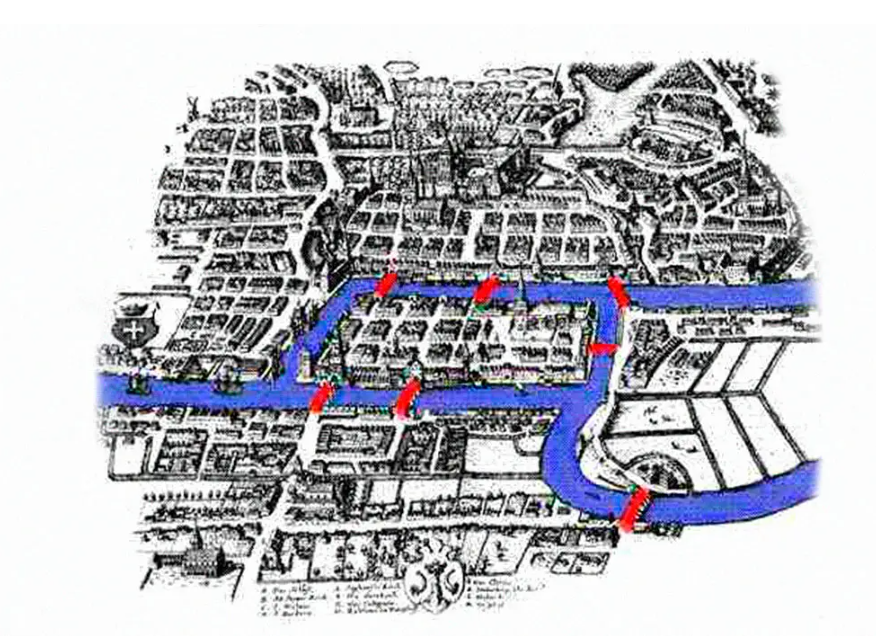
\includegraphics[width=0.6\textwidth]{Ponte de Konigsberg.png}
    \caption{Representação do problema das sete pontes de Königsberg}
    \fonte{Adaptado pelo autor (2026).}
    \label{fig:ponte_konigsberg}
\end{figure}

% ----------------------------------------------------------
\subsection{O Lema do Aperto de Mãos}
\label{subsec:lema_aperto}
% ----------------------------------------------------------

Dessa observação estrutural, derivou-se um dos teoremas mais fundamentais da área, conhecido popularmente como o \textbf{Lema do Aperto de Mãos}.

\begin{lema}[Lema do Aperto de Mãos]
\label{lema:aperto_maos_historico}
  Em qualquer grafo não dirigido $\mathcal{G} = (\mathcal{V},\, \mathcal{A})$, a soma dos graus de todos os vértices é exatamente igual ao dobro do número de arestas:
  \begin{equation}
    \sum_{v \in \mathcal{V}} \delta(v) = 2\,|\mathcal{A}|.
    \label{eq:lema_aperto}
  \end{equation}
\end{lema}

\begin{proof}
  Para compreender essa igualdade, podemos pensar na construção do grafo: cada aresta $\{u, v\}$ liga exatamente dois vértices. Ao desenharmos uma aresta qualquer, ela contribui com uma unidade de grau para o vértice $u$ e outra unidade para o vértice $v$. Portanto, se contarmos as extremidades de todas as arestas existentes, cada aresta terá sido contada exatamente duas vezes — uma vez para cada vértice que ela toca. Como a soma dos graus nada mais é do que o total de extremidades conectadas a todos os vértices, essa soma deve ser, obrigatoriamente, o dobro da quantidade de arestas.
\end{proof}

A analogia que dá nome ao lema é bastante intuitiva: se considerarmos uma festa onde as pessoas (vértices) trocam apertos de mãos (arestas), cada aperto de mão envolve exatamente duas pessoas. Portanto, cada aperto adiciona duas unidades à contagem total de mãos apertadas. Por consequência, a soma total de apertos dados por todas as pessoas será sempre um número par. 

Um corolário direto e fascinante dessa regra --- que serviu de base para diversas provas de complexidade modernas \cite{thomason1978, papadimitriou1994} --- é que, em qualquer reunião, \textbf{o número de pessoas que apertou as mãos de um número ímpar de indivíduos é, obrigatoriamente, par}. No ensino básico, essa propriedade ilustra perfeitamente como relações combinatórias abstratas governam redes de interações reais.

A Figura~\ref{fig:aperto_mao} exemplifica esse resultado em um grafo com cinco vértices, no qual a soma dos graus corresponde exatamente ao dobro do número de arestas.

\begin{figure}[htbp]
    \centering
    \begin{tikzpicture}[
        vertex/.style={circle, draw=black!80, fill=blue!10, very thick, minimum size=8mm, font=\large},
        edge/.style={draw, very thick, black!70}
    ]
        % Vértices com os rótulos de graus
        \node[vertex, label=above:{$\delta=2$}] (v1) at (0,2) {$v_1$};
        \node[vertex, label=right:{$\delta=3$}] (v2) at (2,1) {$v_2$};
        \node[vertex, label=below:{$\delta=2$}] (v3) at (1,-1) {$v_3$};
        \node[vertex, label=below:{$\delta=2$}] (v4) at (-1,-1) {$v_4$};
        \node[vertex, label=left:{$\delta=3$}] (v5) at (-2,1) {$v_5$};
        % Arestas
        \draw[edge] (v1) -- (v2);
        \draw[edge] (v2) -- (v3);
        \draw[edge] (v3) -- (v4);
        \draw[edge] (v4) -- (v5);
        \draw[edge] (v5) -- (v1);
        \draw[edge] (v2) -- (v5); % Aresta interna
    \end{tikzpicture}
    \caption{Grafo ilustrando o Lema do Aperto de Mão}
    \fonte{O autor (2026).}
    \label{fig:aperto_mao}
\end{figure}


% ----------------------------------------------------------
\section{Definições Matemáticas Fundamentais}
% ----------------------------------------------------------

% ----------------------------------------------------------
\subsection{Grafo}
% ----------------------------------------------------------

\begin{definicao}[Grafo]
\label{def:grafo}
  Um \textit{grafo} $\mathcal{G}$ é um par ordenado
  $\mathcal{G} = (\mathcal{V},\, \mathcal{A})$, em que $\mathcal{V}$ é um
  conjunto não vazio de elementos denominados \textit{vértices} (ou nós) e
  $\mathcal{A}$ é um conjunto de pares não ordenados de elementos de
  $\mathcal{V}$, denominados \textit{arestas} \cite{boaventura2009}.
\end{definicao}

De maneira intuitiva, pode-se imaginar um grafo como um diagrama composto por
pontos (os vértices) conectados por linhas (as arestas). Quando dois vértices
estão ligados por uma aresta, diz-se que eles são \textit{adjacentes}
\cite{rosen2012}. A quantidade de vértices de $\mathcal{G}$ é chamada de
\textit{ordem} do grafo, enquanto a quantidade de arestas é chamada de
\textit{tamanho}. A Figura~\ref{fig:representacao_grafo_def} ilustra essa
definição, destacando os vértices $v_i$ e as arestas $e_j$ que os conectam.

\begin{figure}[H] 
    \centering
    \begin{tikzpicture}[
        vertex/.style={circle, draw=black!80, fill=blue!10, very thick, minimum size=8mm, font=\large},
        edge/.style={draw, very thick, black!70}
    ]
        % Vértices
        \node[vertex] (v1) at (0,2) {$v_1$};
        \node[vertex] (v2) at (2.5,0) {$v_2$};
        \node[vertex] (v3) at (0,-2) {$v_3$};
        \node[vertex] (v4) at (-2.5,0) {$v_4$};
        % Arestas
        \draw[edge] (v1) -- (v2) node[midway, above right] {$e_1$};
        \draw[edge] (v2) -- (v3) node[midway, below right] {$e_2$};
        \draw[edge] (v3) -- (v4) node[midway, below left] {$e_3$};
        \draw[edge] (v4) -- (v1) node[midway, above left] {$e_4$};
        \draw[edge] (v1) -- (v3) node[midway, right] {$e_5$};
    \end{tikzpicture}
    \caption{Representação visual de um grafo ilustrando vértices ($v_i$) e arestas ($e_j$)}
    \fonte{O autor (2026).}
    \label{fig:representacao_grafo_def}
\end{figure}

% ----------------------------------------------------------
\subsection{Grau de um Vértice}
% ----------------------------------------------------------

\begin{definicao}[Grau de um vértice]
\label{def:grau}
  O \textit{grau} de um vértice $v$, denotado por $\delta(v)$, corresponde ao
  número de arestas que incidem sobre ele \cite{bondy1976}. Um vértice de grau
  zero é denominado \textit{vértice isolado}.
\end{definicao}

% ----------------------------------------------------------
\subsection{Grafos Não Dirigidos e Grafos Dirigidos}
% ----------------------------------------------------------

\begin{definicao}[Grafo não dirigido e dígrafo]
\label{def:dirigido}
  Um grafo é dito \textit{não dirigido} quando suas arestas não possuem
  orientação, ou seja, a relação entre dois vértices é simétrica. Um
  \textit{grafo dirigido} (ou \textit{dígrafo}) é aquele em que as arestas
  possuem uma orientação definida, representadas por \textit{arcos}; o arco
  $(u, v)$ parte de $u$ e chega em~$v$, sendo distinto do arco $(v, u)$
  \cite{cormen2009}.
\end{definicao}

Em situações práticas do cotidiano, grafos não dirigidos modelam relações
simétricas, como amizades em redes sociais, ao passo que dígrafos modelam
relações assimétricas, como o fluxo de tráfego em vias de mão única ou a
navegação entre páginas da internet \cite{rosen2012}. A Figura~\ref{fig:digrafo}
ilustra um dígrafo em que os arcos direcionados evidenciam essa assimetria.

\begin{figure}[htbp]
    \centering
    \begin{tikzpicture}[
        >={Stealth[scale=1.2]},
        vertex/.style={circle, draw=black!80, fill=red!10, very thick, minimum size=8mm, font=\large},
        edge/.style={->, draw, very thick, black!80}
    ]
        % Vértices
        \node[vertex] (P) at (0,2) {$P$};
        \node[vertex] (Q) at (2.5,2) {$Q$};
        \node[vertex] (R) at (2.5,0) {$R$};
        \node[vertex] (S) at (0,0) {$S$};
        % Arcos direcionados
        \draw[edge] (P) -- (Q);
        \draw[edge] (Q) -- (R);
        \draw[edge] (R) -- (S);
        \draw[edge] (S) -- (P);
        \draw[edge] (P) -- (R);
    \end{tikzpicture}
    \caption{Dígrafo $\mathcal{G}_2$ evidenciando a relação assimétrica e o direcionamento de seus arcos}
    \fonte{O autor (2026).}
    \label{fig:digrafo}
\end{figure}

% ----------------------------------------------------------
\subsection{Subgrafo e Grafo Completo}
% ----------------------------------------------------------

\begin{definicao}[Subgrafo]
  Dado um grafo $\mathcal{G} = (\mathcal{V},\, \mathcal{A})$, um
  \textit{subgrafo} $\mathcal{H}$ de $\mathcal{G}$ é um grafo tal que
  $\mathcal{V}(\mathcal{H}) \subseteq \mathcal{V}(\mathcal{G})$ e
  $\mathcal{A}(\mathcal{H}) \subseteq \mathcal{A}(\mathcal{G})$
  \cite{wilson1996}. 
\end{definicao}

\begin{definicao}[Grafo completo]
\label{def:completo}
  Um grafo é dito \textit{completo} quando todo par de vértices distintos está
  ligado por exatamente uma aresta. O grafo completo com $n$ vértices é
  denotado por $K_n$ \cite{bondy1976}.
\end{definicao}

\begin{teorema}
  O grafo completo $K_n$ possui exatamente $\dfrac{n(n-1)}{2}$ arestas, e
  cada vértice possui grau $n - 1$.
\end{teorema}

\begin{proof}
  Em um grafo completo $K_n$, cada vértice deve se conectar a todos os outros $n-1$ vértices disponíveis no conjunto $\mathcal{V}$. Por essa característica, o grau de qualquer vértice $v$ é exatamente $n-1$. Aplicando agora o Lema do Aperto de Mãos (Lema \ref{lema:aperto_maos_historico}), temos que a soma dos graus é $n \times (n-1)$. Como essa soma equivale ao dobro do número de arestas ($2|\mathcal{A}|$), isolamos $|\mathcal{A}|$:
  \[
    2|\mathcal{A}| = n(n-1) \implies |\mathcal{A}| = \frac{n(n-1)}{2}.
  \]
  Isso confirma que o número de conexões possíveis em um grafo onde todos se ligam é dado por essa fórmula combinatória simples.
\end{proof}

A Figura~\ref{fig:grafo_completo} exibe o grafo completo $K_4$.

\begin{figure}[htbp]
    \centering
    \begin{tikzpicture}[
        vertex/.style={circle, draw=black!80, fill=green!15, very thick, minimum size=8mm, font=\large},
        edge/.style={draw, very thick, black!70}
    ]
        % Posições formando um quadrado/losango
        \node[vertex] (1) at (0,2.5) {$1$};
        \node[vertex] (2) at (2.5,0) {$2$};
        \node[vertex] (3) at (0,-2.5) {$3$};
        \node[vertex] (4) at (-2.5,0) {$4$};
        % Arestas
        \draw[edge] (1) -- (2); 
        \draw[edge] (1) -- (3);
        \draw[edge] (1) -- (4);
        \draw[edge] (2) -- (3); 
        \draw[edge] (2) -- (4);
        \draw[edge] (3) -- (4);
    \end{tikzpicture}
    \caption{Grafo completo $K_4$}
    \fonte{O autor (2026).}
    \label{fig:grafo_completo}
\end{figure}

% ----------------------------------------------------------
\subsection{Caminho, Ciclo e Conectividade}
% ----------------------------------------------------------

\begin{definicao}[Caminho]
  Um \textit{caminho} em um grafo é uma sequência de vértices distintos
  $v_1, v_2, \ldots, v_k$ tal que existe uma aresta entre cada par consecutivo
  $(v_i, v_{i+1})$ \cite{diestel2017}. O número de arestas percorridas é o
  \textit{comprimento} do caminho.
\end{definicao}

\begin{definicao}[Ciclo]
  Um \textit{ciclo} é um caminho fechado, isto é, um caminho em que o primeiro
  e o último vértice coincidem \cite{boaventura2009}. Um grafo sem ciclos é
  denominado \textit{acíclico} ou \textit{floresta}.
\end{definicao}

\begin{definicao}[Grafo conexo]
  Um grafo é denominado \textit{conexo} quando existe pelo menos um caminho
  entre qualquer par de vértices; caso contrário, é dito \textit{desconexo}
  \cite{rosen2012}. As partes maximais conexas de um grafo desconexo são
  chamadas de \textit{componentes conexas}.
\end{definicao}

A Figura~\ref{fig:conectividade} apresenta um grafo desconexo.

\begin{figure}[htbp]
    \centering
    \begin{tikzpicture}[
        vertex/.style={circle, draw=black!80, fill=yellow!15, very thick, minimum size=8mm, font=\large},
        edge/.style={draw, very thick, black!70},
        highlight/.style={draw, line width=2pt, orange} 
    ]
        % Componente 1: Um Ciclo
        \node[vertex] (A) at (0,0) {$A$};
        \node[vertex] (B) at (1,2) {$B$};
        \node[vertex] (C) at (2,0) {$C$};
        \draw[edge] (A) -- (B) -- (C) -- (A);
        % Componente 2: Um Caminho
        \node[vertex] (D) at (4.5,1) {$D$};
        \node[vertex] (E) at (6,0) {$E$};
        \node[vertex] (F) at (7.5,1.5) {$F$};
        \draw[highlight] (D) -- (E) -- (F);
        % Legendas internas
        \node[anchor=north] at (1,-0.5) {Componente 1 (Ciclo)};
        \node[anchor=north] at (6,-0.5) {Componente 2 (Caminho)};
    \end{tikzpicture}
    \caption{Grafo desconexo formado por duas componentes conexas distintas}
    \fonte{O autor (2026).}
    \label{fig:conectividade}
\end{figure}

% ----------------------------------------------------------
\subsection{Caminho e Circuito Euleriano}
\label{sec:euleriano}
% ----------------------------------------------------------

\begin{definicao}[Caminho euleriano e circuito euleriano]
\label{def:euleriano}
  Um \textit{caminho euleriano} é um caminho que percorre cada aresta do grafo
  exatamente uma vez. Um \textit{circuito euleriano} é um caminho euleriano
  que retorna ao vértice de origem \cite{euler1736}.
\end{definicao}

\begin{teorema}[Teorema de Euler]
\label{teo:euler}
  Um grafo conexo admite um circuito euleriano se, e somente se, todos os seus
  vértices possuem grau par. Admite um caminho euleriano (sem ser circuito) se,
  e somente se, possui exatamente dois vértices de grau ímpar
  \cite{diestel2017}.
\end{teorema}

\begin{proof}
  A demonstração clássica baseia-se na ideia de entrada e saída. Se o grafo possui um circuito euleriano, ao percorrê-lo, cada vez que entramos em um vértice por uma aresta, devemos sair por outra aresta distinta (já que não podemos repetir arestas). Isso implica que as arestas incidentes em qualquer vértice que não seja o de início/fim devem ocorrer em pares (uma para entrar, uma para sair). No caso de um circuito, onde o ponto de partida é o mesmo de chegada, todos os vértices — inclusive o inicial — terminam com um número par de incidências. Portanto, a condição de grau par é necessária para garantir que nunca fiquemos ``presos'' em um vértice sem uma aresta de saída disponível.
\end{proof}

A Figura~\ref{fig:euleriano} mostra um exemplo clássico desse resultado.

\begin{figure}[htbp]
    \centering
    \begin{tikzpicture}[
        vertex/.style={circle, draw=black!80, fill=purple!15, very thick, minimum size=6mm, font=\small},
        edge/.style={draw, very thick, black!70}
    ]
        % Vértices
        \node[vertex, label=left:{$\delta=3$}] (A) at (0,0) {};
        \node[vertex, label=right:{$\delta=3$}] (B) at (2.5,0) {};
        \node[vertex, label=left:{$\delta=4$}] (C) at (0,2.5) {};
        \node[vertex, label=right:{$\delta=4$}] (D) at (2.5,2.5) {};
        \node[vertex, label=above:{$\delta=2$}] (E) at (1.25,4) {};
        % Arestas
        \draw[edge] (A) -- (B) -- (D) -- (C) -- (A);
        \draw[edge] (A) -- (D);
        \draw[edge] (B) -- (C);
        \draw[edge] (C) -- (E) -- (D);
    \end{tikzpicture}
    \caption{Grafo em formato de ``envelope'' ou ``casa'', que admite um caminho euleriano mas não um circuito euleriano}
    \fonte{O autor (2026).}
    \label{fig:euleriano}
\end{figure}

% ----------------------------------------------------------
\section{O Ensino de Grafos na Literatura Acadêmica}
% ----------------------------------------------------------

Nesta seção, apresentamos uma breve revisão de trabalhos acadêmicos que discutiram a inserção da Teoria dos Grafos no Ensino Médio. A literatura mostra que, embora o tema ainda seja pouco explorado nos currículos oficiais, há um crescente interesse por parte de pesquisadores em Educação Matemática.

\textcite{malta2008}, em sua dissertação de mestrado, compartilha da ideia de que ``a Teoria dos Grafos apresenta aspectos pertinentes que merecem espaço no currículo da Escola Básica''. A autora apoia-se no contexto histórico para considerar que pertencem à Introdução da Teoria dos Grafos os conceitos que surgiram até o século XVIII, desde \textit{O Problema das Sete Pontes de Königsberg} (1736) até o \textit{Icosian Game} (1856), desenvolvidos por Leonhard Euler e William Hamilton, respectivamente.

Reafirmando a escolha da Metodologia de Resolução de Problemas (\ref{sec:polya}), as \textit{Orientações Educacionais Complementares aos Parâmetros Curriculares Nacionais} (PCN+) enfatizam que a resolução de problemas é peça central para o ensino de Matemática, pois o pensar e o fazer se mobilizam e se desenvolvem quando o indivíduo está engajado ativamente no enfrentamento de desafios \cite{brasil2002}. Essa competência não se desenvolve quando propomos apenas exercícios de aplicação dos conceitos e técnicas matemáticas \cite{brasil2002}.

Adicionalmente, a Lei de Diretrizes e Bases da Educação Nacional (LDB) preconiza que as metodologias de ensino sejam adequadas ao cotidiano discente \cite{brasil1996}. Tal diretriz busca fomentar o pensamento autônomo e a criação de soluções próprias.

Nesse mesmo sentido, \textcite{rodrigues2021} analisam como a inserção de tópicos de Teoria dos Grafos pode favorecer uma formação matemática mais robusta e conectada ao universo digital, alinhando o currículo escolar às demandas da contemporaneidade. Os autores destacam a importância do pensamento computacional e da modelagem de problemas do cotidiano. Ainda sob a ótica da tecnologia, \textcite{silva2020} propõe uma sequência didática para o ensino de grafos no Ensino Médio utilizando o software GeoGebra.

% ----------------------------------------------------------
\subsection{Exemplos Ilustrativos com Representação Gráfica}
% ----------------------------------------------------------

% ----------------------------------------------------------
\subsubsection{Grafo Não Dirigido}
% ----------------------------------------------------------

\label{ex:nao_dirigido}
Considere o grafo $\mathcal{G}_1 = (\mathcal{V}_1,\, \mathcal{A}_1)$ em que
\[
  \mathcal{V}_1 = \{A,\, B,\, C,\, D,\, E\}
  \quad \text{e} \quad
  \mathcal{A}_1 = \{AB,\, AC,\, AD,\, BC,\, CD,\, DE,\, EA\}.
\]

Esse grafo possui $|\mathcal{V}_1| = 5$ vértices e $|\mathcal{A}_1| = 7$
arestas. Aplicando o Lema do Aperto de Mãos
(Lema~\ref{lema:aperto_maos_historico}), a soma dos graus deve ser $2 \times 7 = 14$. De fato: $\delta(A) = 4$, $\delta(B) = 2$, $\delta(C) = 3$, $\delta(D) = 3$,
$\delta(E) = 2$, totalizando $4 + 2 + 3 + 3 + 2 = 14$ \checkmark

A Figura~\ref{fig:grafo_nao_dirigido} apresenta a representação gráfica desse
grafo não dirigido.

\begin{figure}[htb]
  \centering
  \begin{tikzpicture}[
      vertex/.style = {circle, draw, fill=blue!20,
                       minimum size=1.2cm, font=\sffamily\bfseries},
      edge/.style   = {thick}
  ]
    \node[vertex] (A) at (0,0)    {$A$};
    \node[vertex] (B) at (3,1)    {$B$};
    \node[vertex] (C) at (4,-2)   {$C$};
    \node[vertex] (D) at (1,-2.5) {$D$};
    \node[vertex] (E) at (-1,-1)  {$E$};
    \draw[edge] (A) -- (B);
    \draw[edge] (A) -- (C);
    \draw[edge] (A) -- (D);
    \draw[edge] (B) -- (C);
    \draw[edge] (C) -- (D);
    \draw[edge] (D) -- (E);
    \draw[edge] (E) -- (A);
\end{tikzpicture}
  \caption{Grafo não dirigido $\mathcal{G}_1$ com 5 vértices e 7 arestas}
  \fonte{O autor (2026).}
  \label{fig:grafo_nao_dirigido}
\end{figure}

Esse grafo pode modelar, por exemplo, um mapa rodoviário simplificado em que os
vértices representam cidades e as arestas representam estradas de mão dupla que
as interligam \cite{jurkiewicz2007}. Verifique ainda que $\delta(A) = 4$ e
$\delta(B) = \delta(E) = 2$ são pares, enquanto $\delta(C) = \delta(D) = 3$
são ímpares; há exatamente dois vértices de grau ímpar, logo $\mathcal{G}_1$
admite caminho euleriano, mas não circuito euleriano
(Teorema~\ref{teo:euler}).

% ----------------------------------------------------------
\subsubsection{Grafo Dirigido (Dígrafo)}
% ----------------------------------------------------------

\label{ex:digrafo}
Considere o dígrafo $\mathcal{G}_2 = (\mathcal{V}_2,\, \mathcal{A}_2)$ em que
\[
  \mathcal{V}_2 = \{P,\, Q,\, R,\, S\}
  \quad \text{e} \quad
  \mathcal{A}_2 = \{(P,Q),\, (Q,R),\, (R,S),\, (S,P),\, (P,R)\}.
\]
Os arcos possuem direção. A Figura~\ref{fig:digrafo_ex2}
representa graficamente esse dígrafo.

\begin{figure}[htb]
  \centering
  \begin{tikzpicture}[
      vertex/.style  = {circle, draw, fill=orange!25,
                        minimum size=1.2cm, font=\sffamily\bfseries},
      arc/.style     = {thick, -{Stealth[length=7pt]}},
      node distance  = 3cm
  ]
    \node[vertex] (P) at (0,0)   {$P$};
    \node[vertex] (Q) at (3,0)   {$Q$};
    \node[vertex] (R) at (3,-3)  {$R$};
    \node[vertex] (S) at (0,-3)  {$S$};
    \draw[arc] (P) -- (Q);
    \draw[arc] (Q) -- (R);
    \draw[arc] (R) -- (S);
    \draw[arc] (S) -- (P);
    \draw[arc] (P) -- (R);
\end{tikzpicture}
  \caption{Dígrafo $\mathcal{G}_2$ com 4 vértices e 5 arcos orientados}
  \fonte{O autor (2026).}
  \label{fig:digrafo_ex2}
\end{figure}

Essa estrutura é adequada para modelar vias de mão única em uma cidade ou o
fluxo de informações em uma rede de computadores \cite{cormen2009}. A distinção
entre grafos dirigidos e não dirigidos será explorada no Apêndice~\ref{apendice:redes}.

% ----------------------------------------------------------
\subsubsection{Grafo Completo $K_4$}
% ----------------------------------------------------------

\label{ex:k4}
O grafo completo $K_4$ possui $n = 4$ vértices e
$\dfrac{4 \times 3}{2} = 6$ arestas, sendo todo par de vértices adjacente.
Todos os vértices possuem grau $\delta = n - 1 = 3$ \cite{bondy1976}.

Os grafos completos são frequentemente utilizados como casos-limite em problemas
de otimização combinatória, como o clássico Problema do Caixeiro Viajante, que
busca o menor caminho que passa por todos os vértices exatamente uma vez
\cite{rosen2012}. Esse problema é retomado na proposta didática do Apêndice~\ref{apendice:caixeiro}.
A Figura~\ref{fig:k4} ilustra o grafo completo $K_4$.

\begin{figure}[!t]
  \centering
  \begin{tikzpicture}[
      vertex/.style = {circle, draw, fill=green!25,
                       minimum size=1.2cm, font=\sffamily\bfseries},
      edge/.style   = {thick}
  ]
    \node[vertex] (1) at (0, 2)   {$1$};
    \node[vertex] (2) at (2, 0)   {$2$};
    \node[vertex] (3) at (0,-2)   {$3$};
    \node[vertex] (4) at (-2, 0)  {$4$};
    \draw[edge] (1) -- (2);
    \draw[edge] (1) -- (3);
    \draw[edge] (1) -- (4);
    \draw[edge] (2) -- (3);
    \draw[edge] (2) -- (4);
    \draw[edge] (3) -- (4);
\end{tikzpicture}
  \caption{Grafo completo $K_4$ com 4 vértices e 6 arestas}
  \fonte{O autor (2026).}
  \label{fig:k4}
\end{figure}
\vfill

% ==========================================================
\chapter{ANÁLISE DOCUMENTAL: A TEORIA DOS GRAFOS E A BNCC}
\label{cap:bncc}
% ==========================================================

Investigar a relevância da Teoria dos Grafos no contexto da Educação Básica e
sua relação com as competências e habilidades previstas na BNCC é essencial para
justificar sua inserção curricular. Este capítulo analisa a Base Nacional Comum
Curricular (BNCC) e documentos complementares, identificando pontos de
articulação com os conceitos de grafos apresentados no capítulo anterior.

% ----------------------------------------------------------
\section{A Matemática Discreta no Ensino Médio}
% ----------------------------------------------------------

A Matemática Discreta, da qual a Teoria dos Grafos é um dos ramos mais
proeminentes, tradicionalmente tem pouco espaço no currículo do Ensino Médio
brasileiro, que prioriza áreas como Álgebra, Geometria e Análise (Cálculo
diferencial e integral elementar). No entanto, a BNCC, ao propor a formação
integral do estudante e o desenvolvimento de competências para o século XXI,
abre espaço para a inclusão de tópicos de Matemática Discreta.

O documento oficial destaca a importância de o estudante ``identificar e
representar relações de interdependência entre grandezas, modelizar situações
diversas e resolver problemas que envolvem contagens, arranjos, combinações e
probabilidades'' \cite{brasil2018}. Embora mencione explicitamente análise
combinatória, a Teoria dos Grafos aparece como um desdobramento natural desses
estudos, fornecendo uma linguagem visual e relacional para problemas de
otimização e conectividade.

Além disso, as competências específicas de Matemática para o Ensino Médio, como
``utilizar estratégias, conceitos e procedimentos matemáticos para interpretar
situações em diversos contextos'' e ``propor ou participar de ações para
investigar desafios do mundo contemporâneo'', alinham-se perfeitamente à
abordagem por meio de grafos.

\subsection{Relevância da Teoria dos Grafos na Educação Básica}

A investigação da relevância da Teoria dos Grafos no contexto da Educação Básica e sua relação com as competências e habilidades previstas na BNCC revela que ela é uma ferramenta poderosa para modelar e resolver problemas do cotidiano. Sua inclusão no currículo pode proporcionar uma abordagem mais prática e aplicada de conceitos matemáticos, permitindo que os alunos desenvolvam habilidades críticas e analíticas. A Base Nacional Comum Curricular (BNCC) \cite{brasil2018} enfatiza a importância de desenvolver competências que preparem os alunos para enfrentar desafios do mundo real.

A Teoria dos Grafos pode ser utilizada para:

\begin{itemize}
    \item Promover o pensamento algorítmico e computacional defendido pela BNCC. Oferecendo uma linguagem matemática que pode ser utilizada para resolver problemas complexos, como otimização de rotas e análise de redes.
    \item Integrar-se a diversas disciplinas, como Ciências, Geografia e História, permitindo uma aprendizagem mais contextualizada e significativa.
\end{itemize}

\subsection{Estratégias Didáticas para a Introdução de Grafos}

Discutir potenciais estratégias didáticas para a introdução dos conceitos de grafos no Ensino Médio, com foco em abordagens interdisciplinares e contextualizadas, mostra que a resolução de problemas ligados ao cotidiano é uma das maneiras mais eficientes de se abordar o assunto. Isso corrobora a recomendação de dar ``ênfase na resolução de problemas, na exploração da Matemática a partir dos problemas vividos no cotidiano e encontrados nas várias disciplinas'' \cite{brasil2002}.

Adicionalmente, a LDB (Lei de Diretrizes e Bases da Educação Nacional) preconiza que as metodologias de ensino sejam adequadas ao cotidiano discente \cite{brasil1996}. Tal diretriz busca fomentar o pensamento autônomo e a criação de soluções próprias, permitindo que o estudante desenvolva independência na capacidade de resolver problemas.

Assim como ocorreu em outros estados, a Bahia vem incorporando atualizações importantes em suas diretrizes, fruto do trabalho coletivo de professores e equipes técnicas. Segundo o referencial da Educação do Estado da Bahia \cite{bahia2019}, propõem-se estratégias que ampliam o repertório matemático dos estudantes, incluindo temas que raramente aparecem no currículo tradicional, como elementos introdutórios da Teoria dos Grafos.

Como visto anteriormente, a Teoria dos Grafos foi formulada a partir de um problema. Logo, acreditamos que a metodologia de Resolução de Problemas pode ser utilizada para a abordagem de Grafos no Ensino Médio. Reafirmando a escolha desse caminho, as Orientações Educacionais Complementares aos Parâmetros Curriculares Nacionais (PCN+) enfatizam que a resolução de problemas é peça central para o ensino de Matemática, pois o pensar e o fazer se mobilizam e se desenvolvem quando o indivíduo está engajado ativamente no enfrentamento de desafios.

\begin{quote}
\small
Essa competência não se desenvolve quando propomos apenas exercícios de aplicação dos conceitos e técnicas matemáticas, pois, neste caso, o que está em ação é uma simples transposição analógica: o aluno busca na memória um exercício semelhante e desenvolve passos análogos aos daquela situação, o que não garante que seja capaz de utilizar seus conhecimentos em situações diferentes ou mais complexas \cite{brasil2002}.
\end{quote}

% ----------------------------------------------------------
\section{Relação com as Competências e Habilidades da BNCC}
% ----------------------------------------------------------

A Base Nacional Comum Curricular (BNCC) \cite{brasil2018} enfatiza a importância de desenvolver competências que preparem os alunos para enfrentar desafios do mundo real. Os conceitos formalizados no Capítulo~\ref{cap:fundamentos} e operacionalizados nas atividades do Capítulo~\ref{cap:proposta} articulam-se diretamente com diversas habilidades requeridas pelo documento. 

Podemos destacar as seguintes habilidades:

\begin{itemize}
  \item \textbf{EM13MAT101}: ``Interpretar situações econômicas, sociais e científicas por meio de gráficos, tabelas e medidas, identificando relações de dependência e representando-as por meio de modelos matemáticos''. A modelagem de redes sociais, rotas de transporte e problemas de conexão atende diretamente a essa habilidade.
  \item \textbf{EM13MAT201}: ``Propor e testar estratégias de resolução de problemas de contagem que envolvem agrupamentos ordenáveis ou não ordenáveis, de modo a construir e aplicar os conceitos de arranjo, combinação e permutação''. O Problema do Caixeiro Viajante (Seção \ref{sub:proposta_caixeiro}) e a contagem de rotas são exemplos concretos. 
  \item \textbf{EM13MAT307}: ``Empregar diferentes estratégias para resolver problemas envolvendo a determinação de um percurso ou a organização de um circuito, considerando condições de adjacência, conectividade e otimização''. Essa habilidade é praticamente uma descrição do estudo de caminhos e circuitos eulerianos.
  \item \textbf{EM13MAT315}: ``Utilizar conhecimentos matemáticos para compreender e atuar no mundo digital, aplicando conceitos de algoritmos, pensamento computacional e modelagem''. A Teoria dos Grafos é fundamental para algoritmos de busca e sistemas de recomendação.
  \item \textbf{EM13MAT401}: ``Converter representações algébricas de funções polinomiais de 1º grau para representações geométricas no plano cartesiano, distinguindo os casos nos quais o comportamento é proporcional, recorrendo ou não a softwares ou aplicativos de álgebra e geometria dinâmica''. O estudo de grafos enriquece a visualização estrutural dessas relações e do pensamento analítico.
\end{itemize}

% ----------------------------------------------------------
\section{O Pensamento Computacional e a Interdisciplinaridade}
\label{sec:interdisciplinaridade}
% ----------------------------------------------------------

A BNCC defende a promoção do pensamento algorítmico e computacional, e a Teoria dos Grafos oferece uma linguagem matemática ideal para resolver problemas complexos, como a otimização de rotas e a análise de redes \cite{lima2022}. Ela fornece a base teórica perfeita para ensinar esses conceitos sem a necessidade imediata de computadores, mas servindo de ponte estruturada para atividades tecnológicas mais avançadas.

Além disso, a interdisciplinaridade é um princípio estruturante do Novo Ensino Médio. A aplicação da Teoria dos Grafos pode ser integrada a diversas disciplinas, permitindo uma aprendizagem mais contextualizada e significativa. A seguir, detalhamos alguns exemplos:

\begin{itemize}
  \item \textbf{Geografia e História}: 
    Os grafos são ferramentas fundamentais para o estudo de rotas comerciais históricas (como a Rota da Seda ou as navegações portuguesas), permitindo visualizar a interconexão entre diferentes impérios e cidades. Em Geografia, a modelagem de redes de transporte, fluxos migratórios ou a propagação de fenômenos climáticos (como o deslocamento de frentes frias) pode ser representada por grafos, onde os vértices são cidades ou regiões e as arestas indicam vias ou rotas de deslocamento. Essa abordagem ajuda os alunos a compreender a importância da localização e da conectividade no desenvolvimento econômico e social.

  \item \textbf{Ciências e Biologia}: 
    Na Biologia, as cadeias alimentares e as teias tróficas são exemplos clássicos de grafos dirigidos: os vértices representam espécies e as arestas orientadas indicam o fluxo de energia (quem come quem). Em Epidemiologia, a propagação de doenças em uma população pode ser simulada por meio de grafos, onde os vértices são indivíduos ou regiões e as arestas representam contatos ou rotas de transmissão. Essa modelagem permite entender conceitos como a velocidade de contágio e a eficácia de medidas de isolamento, conectando a Matemática a questões de saúde pública atuais.

  \item \textbf{Língua Portuguesa}: 
    A análise de redes semânticas é um campo fértil para a aplicação de grafos: as palavras (vértices) podem ser ligadas por relações de sinonímia, antonímia, hiperonímia, ou por coocorrência em textos. Em literatura, pode-se construir um grafo de personagens de um romance, onde as arestas indicam interações ou diálogos, revelando a estrutura da trama e os personagens centrais. Além disso, a organização de textos argumentativos pode ser mapeada como um grafo de ideias, mostrando como os argumentos se conectam e sustentam a tese principal, desenvolvendo a capacidade de estruturação lógica da escrita.
\end{itemize}

O cruzamento dessas áreas mostra ao estudante como a Matemática atua como uma linguagem universal para a resolução de problemas complexos que extrapolam os limites exatos da disciplina.

% ==========================================================
\chapter{PROPOSTA DIDÁTICA PARA O ENSINO DE GRAFOS}
\label{cap:proposta}
% ==========================================================

Os capítulos anteriores construíram dois pilares complementares: o Capítulo~\ref{cap:fundamentos} estabeleceu o arcabouço matemático formal da Teoria dos Grafos e revisou a literatura pertinente, enquanto o Capítulo~\ref{cap:bncc} analisou as conexões desse tema com as diretrizes curriculares. O presente capítulo traduz esses pilares em uma proposta de ensino coerente, progressiva e metodologicamente fundamentada, apresentando a metodologia adotada, a descrição das propostas de atividades, sugestões de sequência didática e uma discussão sobre os desafios de implementação.

% ----------------------------------------------------------
\section{Metodologia de Resolução de Problemas}
\label{sec:metodologia}
% ----------------------------------------------------------

A resolução de problemas ligados ao cotidiano é uma das maneiras mais adequadas para se abordar a Teoria dos Grafos no Ensino Médio. As Orientações Educacionais Complementares aos Parâmetros Curriculares Nacionais (PCN+) enfatizam que a resolução de problemas é peça central para o ensino de Matemática, pois o pensar e o fazer se mobilizam e se desenvolvem quando o indivíduo está engajado ativamente no enfrentamento de desafios \cite{brasil2002}. Essa competência não se desenvolve quando propomos apenas exercícios de aplicação, pois, nesse caso, o que está em ação é uma simples transposição analógica, sem garantia de transferência para situações novas \cite{brasil2002}.

Nessa perspectiva, cada atividade apresentada a seguir foi deliberadamente estruturada para: (i) partir de um problema concreto e motivador; (ii) conduzir o estudante à formalização gradual dos conceitos do Capítulo~\ref{cap:fundamentos}; e (iii) promover a generalização e a reflexão sobre o resultado obtido. As etapas seguem o modelo proposto por \textcite{polya2006}, discutido na Seção \ref{sec:polya}.

Adicionalmente, a Lei de Diretrizes e Bases da Educação Nacional (LDB) preconiza que as metodologias de ensino sejam adequadas ao cotidiano discente \cite{brasil1996}, buscando fomentar o pensamento autônomo e a criação de soluções próprias. Por isso, as atividades utilizam contextos como redes sociais, rotas de entrega e organização de um bairro, que são situações familiares aos jovens.

% ----------------------------------------------------------
\section{Propostas Didáticas}
\label{sec:propostas_didaticas}
% ----------------------------------------------------------

Nesta seção, são apresentadas as propostas didáticas que constituem o núcleo prático desta pesquisa, estruturadas como alternativas pedagógicas para a introdução da Teoria dos Grafos no Ensino Médio. Cada proposta é discutida aqui sob o ponto de vista de sua fundamentação e objetivos gerais, enquanto as respectivas fichas de atividades (prontas para aplicação) e seus gabaritos detalhados estão localizados nos Apêndices deste trabalho.

\subsection{Proposta I --- A Vila dos Grafos: construindo e analisando um grafo}
\label{sub:proposta_vila}

Esta primeira proposta, cujo material completo de aplicação encontra-se no Apêndice~\ref{apendice:vila}, tem como objetivo introduzir os conceitos mais elementares da Teoria dos Grafos --- vértices, arestas e graus --- por meio de um problema clássico de modelagem e planejamento urbano.

A abordagem escolhida permite que o aluno faça a transição do pensamento concreto (um mapa viário) para a representação matemática abstrata (o grafo). O problema convida os estudantes a atuarem como engenheiros de trânsito responsáveis por mapear as ruas de um bairro fictício. Ao desenharem as conexões entre os locais, eles constroem o grafo intuitivamente.

A partir dessa construção, a atividade avança para a formalização, exigindo a listagem dos conjuntos de vértices e arestas, e o cálculo do grau de cada ponto. O ponto alto da proposta é a verificação experimental do Lema do Aperto de Mãos. Em vez de receberem a fórmula pronta de que a soma dos graus é igual ao dobro do número de arestas, os alunos são levados a calcular essa soma, comparar com o mapa desenhado e deduzir a lógica geométrica por trás da relação (o fato de que cada rua possui duas extremidades). Essa estratégia transforma a sala de aula em um ambiente de experimentação, desenvolvendo a argumentação matemática e o raciocínio dedutivo.

\subsection{Proposta II --- Redes Sociais e Conectividade}
\label{sub:proposta_redes}

A segunda proposta, vinculada ao roteiro de aplicação disponível no Apêndice~\ref{apendice:redes}, utiliza um cenário altamente familiar e atrativo para os jovens da atualidade: a dinâmica das redes sociais. O objetivo é explorar a diferença estrutural entre relações simétricas e assimétricas, introduzindo formalmente os conceitos de grafos não dirigidos e dígrafos (grafos dirigidos).

A atividade propõe a análise de um grupo de amigos inseridos em duas plataformas distintas: uma que exige adição mútua para criar um vínculo (semelhante ao Facebook ou WhatsApp) e outra baseada em seguidores unidirecionais (como o X/Twitter ou Instagram). Os alunos precisam representar a primeira rede sem o uso de setas e a segunda utilizando arcos direcionados, calculando, em seguida, os graus de entrada e saída.

Essa contextualização cumpre um papel fundamental: demonstrar que a Matemática não se resume a números e equações geométricas, mas é uma linguagem poderosa para modelar o fluxo de informações e as interações humanas no ambiente digital. A atividade estimula a percepção crítica sobre como os algoritmos e as regras de negócio das plataformas de tecnologia são intrinsecamente baseados em estruturas de grafos.

\subsection{Proposta III --- O Problema do Caixeiro Viajante Simplificado}
\label{sub:proposta_caixeiro} 

A terceira proposta, cujo instrumental pedagógico estende-se no Apêndice~\ref{apendice:caixeiro}, eleva o nível de abstração ao introduzir a otimização de rotas por meio do clássico Problema do Caixeiro Viajante (PCV). O foco desta atividade é aplicar a Teoria dos Grafos no campo da logística, abordando grafos completos e arestas ponderadas (com pesos representando distâncias).

O cenário apresenta um entregador que precisa visitar quatro cidades exatas e retornar ao ponto de origem gastando o mínimo de quilometragem possível. Inicialmente, o problema parece simples, permitindo que os alunos listem todas as permutações de rotas manualmente e calculem o custo de cada uma para encontrar a menor distância.

No entanto, o verdadeiro valor pedagógico da proposta surge na última etapa, quando os alunos são questionados sobre o que aconteceria se o número de cidades fosse ampliado para dez. Ao utilizarem a análise combinatória básica (cálculo de fatorial) para descobrir que haveria mais de 360 mil rotas possíveis, os estudantes vivenciam o fenômeno da explosão combinatória.

Essa reflexão final é crucial para o desenvolvimento do pensamento computacional. Ela ilustra de forma impactante os limites da resolução por ``força bruta'' e justifica a necessidade do desenvolvimento de algoritmos e heurísticas na Ciência da Computação e na Matemática Aplicada para resolver problemas do mundo real, conectando o currículo da Educação Básica a desafios científicos contemporâneos.

% ----------------------------------------------------------
\section{Sequência Didática Sugerida}
\label{sec:sequencia_didatica}
% ----------------------------------------------------------

Com base na articulação entre os fundamentos matemáticos (Capítulo~\ref{cap:fundamentos}), a análise documental (Capítulo~\ref{cap:bncc}) e as atividades propostas, sugere-se a seguinte sequência didática de quatro encontros:

\begin{enumerate}
  \item \textbf{1º encontro --- Introdução e motivação histórica:} apresentação do problema das Pontes de Königsberg como motivação histórica e como situação-problema aberta. O professor conduz uma discussão coletiva antes de formalizar a Definição~\ref{def:grafo}.
  \item \textbf{2º encontro --- Construindo grafos:} realização da Proposta I (Apêndice~\ref{apendice:vila}), que mobiliza as Definições~\ref{def:grafo} e \ref{def:grau}, além do Lema~\ref{lema:aperto_maos_historico}. O professor sistematiza o Lema do Aperto de Mãos ao final.
  \item \textbf{3º encontro --- Redes e sentidos:} discussão sobre grafos dirigidos e não dirigidos por meio da Proposta II (Apêndice~\ref{apendice:redes}). Retoma-se o Teorema~\ref{teo:euler} como fechamento da discussão sobre caminhos e circuitos.
  \item \textbf{4º encontro --- Otimização e síntese:} realização da Proposta III (Apêndice~\ref{apendice:caixeiro}), destacando a conexão com o pensamento computacional e a explosão combinatória. O encontro encerra-se com uma reflexão sobre a presença dos grafos em aplicativos de navegação, redes sociais e outros contextos digitais.
\end{enumerate}

Recomenda-se, ao longo dos encontros, o uso de recursos digitais como o GeoGebra \cite{silva2020}, que permite a construção interativa de grafos e favorece a aprendizagem visual e exploratória.

% ----------------------------------------------------------
\section{Desafios e Limitações na Implementação na Rede Pública}
% ----------------------------------------------------------

A inserção de novos conteúdos matemáticos na rede pública esbarra primeiramente na defasagem de base dos estudantes. O distanciamento histórico em relação à álgebra e à aritmética elementar costuma gerar resistência a tópicos adicionais. Contudo, a Teoria dos Grafos tem o potencial de contornar parte desse obstáculo pedagógico devido ao seu forte caráter visual. Em vez de exigir a manipulação imediata de equações ou fórmulas complexas, a modelagem geométrica por meio de vértices e arestas permite que o aluno engaje na resolução do problema de forma mais intuitiva, atenuando a ansiedade frequentemente observada nas aulas de Matemática.

Do ponto de vista do planejamento docente, o principal entrave é a quase total escassez de materiais didáticos sobre grafos voltados para o Ensino Médio em língua portuguesa. A literatura disponível concentra-se massivamente no ensino superior. Sem um material de apoio contextualizado, o professor regente --- muitas vezes já sobrecarregado pela rotina de múltiplas turmas e exigências curriculares --- precisaria adaptar todo o conteúdo por conta própria. A estruturação das propostas didáticas detalhadas nos apêndices deste trabalho surge como uma alternativa para minimizar esse obstáculo, oferecendo um roteiro de aplicação direto que poupa o tempo de preparação do professor.

Outro fator estrutural limitante é a infraestrutura tecnológica das escolas. Embora a Matemática Discreta seja o alicerce da Ciência da Computação, o desenvolvimento do pensamento computacional nas escolas públicas esbarra frequentemente na falta de laboratórios de informática funcionais. As atividades propostas lidam com essa restrição ao adotar a abordagem da ``Computação Desplugada''. Ao mapear redes ou otimizar rotas usando apenas lápis e papel, os alunos simulam a lógica dos algoritmos. Eles exercitam a decomposição de problemas e a análise combinatória sem depender, em momento algum, de equipamentos eletrônicos ou acesso à internet.

A carga horária regular da disciplina de Matemática também impõe restrições severas. A execução de problemas investigativos, que demandam tempo para tentativa, erro e discussão, é difícil de ser esgotada nos curtos períodos tradicionais de aula. Diante disso, a aplicação desta proposta encontra maior viabilidade nos espaços flexíveis do currículo, como as disciplinas eletivas, trilhas de aprofundamento ou clubes de ciências, especialmente no contexto das escolas de tempo integral, onde a matriz horária permite uma abordagem mais horizontal e menos corrida.

Nestas circunstâncias de aplicação, o apoio logístico em sala de aula torna-se decisivo. A implementação de metodologias ativas com turmas numerosas ganha muita tração quando há a presença de acadêmicos vinculados a programas de iniciação à docência. Os futuros docentes, ao atuarem como comediadores nas atividades, viabilizam um acompanhamento mais próximo aos grupos de alunos. Essa colaboração direta divide a carga de mediação com o professor titular, tornando a inserção de temas inovadores uma meta atingível e realista na educação pública.

% ==========================================================
\chapter{Considerações finais}
% ==========================================================

% ----------------------------------------------------------

Este trabalho teve como objetivo central investigar e propor caminhos viáveis para a inserção teórica da Teoria dos Grafos no currículo de Matemática do Ensino Médio da rede pública de ensino. Partindo da premissa de que a educação matemática deve dialogar com a complexidade do mundo contemporâneo, a pesquisa evidenciou que a Matemática Discreta não precisa --- e não deve --- ficar restrita aos bancos de dados universitários.

Ao longo da análise documental, constatou-se que a Teoria dos Grafos possui um alinhamento natural e profundo com as competências exigidas pela Base Nacional Comum Curricular (BNCC). Mais do que cumprir uma exigência normativa, o estudo de vértices, arestas e caminhos mostrou-se uma ferramenta poderosa para o desenvolvimento do pensamento computacional. Por meio da abordagem da ``Computação Desplugada'', demonstrou-se que é perfeitamente possível ensinar aos jovens a lógica dos algoritmos, a otimização de rotas e a estruturação de dados sem a dependência de laboratórios de informática, superando uma das grandes barreiras estruturais das escolas públicas.

As três propostas didáticas elaboradas neste estudo --- focadas em planejamento urbano (A Vila dos Grafos), dinâmica de redes sociais e o Problema do Caixeiro Viajante --- traduzem o rigor formal da Matemática em situações-problema do cotidiano discente. A adoção da Metodologia de Resolução de Problemas permitiu estruturar um material que não apenas transmite fórmulas, mas convida o aluno a investigar, errar, testar e deduzir relações lógicas, como o Lema do Aperto de Mãos e a explosão combinatória.

Reconhecemos que a transposição didática desse conteúdo para o chão da escola pública esbarra em desafios crônicos, como a defasagem matemática de base, a escassez de materiais em língua portuguesa e a sobrecarga da carga horária. No entanto, o trabalho evidenciou que essas barreiras podem ser mitigadas por meio da colaboração. A presença ativa de programas de iniciação à docência, como o PIBID, atuando em conjunto com os professores regentes, é fundamental para viabilizar metodologias ativas e garantir um acompanhamento próximo e humano aos estudantes.

Por se tratar de uma pesquisa de natureza qualitativa e documental, este estudo não se encerra em si mesmo, mas atua como um ponto de partida. Como encaminhamento para trabalhos futuros, sugere-se a aplicação prática das sequências didáticas aqui propostas em turmas reais do Ensino Médio, preferencialmente em escolas de tempo integral. A coleta empírica de dados sobre a recepção dos alunos e as estratégias de raciocínio por eles adotadas enriquecerá ainda mais o debate.

Espera-se que esta monografia sirva como um recurso de apoio sólido para professores e futuros docentes que desejam inovar em suas práticas. Ao modelarmos o mundo através de grafos, mostramos aos estudantes que a Matemática é, acima de tudo, a linguagem das conexões.

% ----------------------------------------------------------
% ELEMENTOS PÓS-TEXTUAIS
% ----------------------------------------------------------
\postextual

\printbibliography

% ---
% Apêndices
% ---
\begin{apendicesenv}
\partapendices

% ==========================================
% APÊNDICE A — Proposta I: A Vila dos Grafos
% ==========================================
\chapter{Proposta I --- A Vila dos Grafos}
\label{apendice:vila}

% ----------------------------------------------------------
\section{Ficha de atividade para o aluno}
% ----------------------------------------------------------

\textbf{Orientações iniciais:} Leia o problema com atenção e responda às questões. Use lápis para desenhar o grafo e, se necessário, borracha para corrigir.

\medskip

\textbf{Leia o problema:}

Você é o engenheiro de trânsito responsável por mapear o centro de um pequeno bairro chamado ``Vila dos Grafos''. Neste bairro, existem 5 pontos de grande importância: A (Prefeitura), B (Escola), C (Padaria), D (Praça Central) e E (Hospital). Para conectar esses locais, existem 7 ruas de mão dupla:

\begin{enumerate}[noitemsep]
  \item Prefeitura (A) $\leftrightarrow$ Escola (B)
  \item Prefeitura (A) $\leftrightarrow$ Praça Central (D)
  \item Escola (B) $\leftrightarrow$ Padaria (C)
  \item Escola (B) $\leftrightarrow$ Praça Central (D)
  \item Padaria (C) $\leftrightarrow$ Praça Central (D)
  \item Padaria (C) $\leftrightarrow$ Hospital (E)
  \item Praça Central (D) $\leftrightarrow$ Hospital (E)
\end{enumerate}

\textbf{1.} Desenhe o mapa do bairro representando os locais como pontos (vértices) e as ruas como linhas (arestas).

\vspace{4cm}

\textbf{2.} Liste o conjunto de vértices e o conjunto de arestas. Quantos vértices e quantas arestas o grafo possui?

\vspace{0.3cm}
\noindent\rule{\textwidth}{0.4pt}\vspace{0.3cm}
\noindent\rule{\textwidth}{0.4pt}\vspace{0.3cm}
\noindent\rule{\textwidth}{0.4pt}

\textbf{3.} Calcule o grau de cada vértice (ou seja, quantas ruas se conectam a cada local).

\vspace{0.3cm}
\noindent\rule{\textwidth}{0.4pt}\vspace{0.3cm}
\noindent\rule{\textwidth}{0.4pt}\vspace{0.3cm}
\noindent\rule{\textwidth}{0.4pt}

\textbf{4.} Some todos os graus obtidos na questão 3 e compare com o número total de arestas. O que você conclui? Explique a relação matemática.

\vspace{0.3cm}
\noindent\rule{\textwidth}{0.4pt}\vspace{0.3cm}
\noindent\rule{\textwidth}{0.4pt}\vspace{0.3cm}
\noindent\rule{\textwidth}{0.4pt}\vspace{0.3cm}
\noindent\rule{\textwidth}{0.4pt}

\newpage
% ----------------------------------------------------------
\section{Gabarito comentado}
% ----------------------------------------------------------

\textbf{Questão 1 – Representação gráfica esperada:}

O aluno deve desenhar cinco pontos (A, B, C, D, E) e ligá-los com as arestas correspondentes. A figura abaixo mostra o grafo correto (não se preocupe com a posição exata dos pontos, desde que as conexões sejam as mesmas).

\begin{center}
\begin{tikzpicture}[
    node distance=2.5cm and 3.5cm,
    vertex/.style={circle, draw=blue!70!black, fill=blue!10, very thick, minimum size=1.2cm, align=center, font=\small\bfseries},
    centervertex/.style={circle, draw=orange!80!black, fill=orange!20, very thick, minimum size=1.2cm, align=center, font=\small\bfseries},
    edge/.style={draw, very thick, black!70}
]
    \node[centervertex] (D) {D \\ Praça};
    \node[vertex] (A) [above left=of D] {A \\ Pref.};
    \node[vertex] (B) [above right=of D] {B \\ Escola};
    \node[vertex] (C) [below right=of D] {C \\ Padaria};
    \node[vertex] (E) [below left=of D] {E \\ Hosp.};
    \draw[edge] (A) -- (B);
    \draw[edge] (A) -- (D);
    \draw[edge] (B) -- (C);
    \draw[edge] (B) -- (D);
    \draw[edge] (C) -- (D);
    \draw[edge] (C) -- (E);
    \draw[edge] (D) -- (E);
\end{tikzpicture}
\end{center}

\textbf{Questão 2 – Conjuntos:}
\[
\mathcal{V} = \{A, B, C, D, E\},\quad
\mathcal{A} = \{AB, AD, BC, BD, CD, CE, DE\}.
\]
O grafo tem 5 vértices e 7 arestas.

\textbf{Questão 3 – Graus:}
\[
\delta(A)=2,\quad \delta(B)=3,\quad \delta(C)=3,\quad \delta(D)=4,\quad \delta(E)=2.
\]

\textbf{Questão 4 – Soma dos graus:}
\[
2+3+3+4+2 = 14,
\]
que é exatamente o dobro do número de arestas (7). Isso confirma o Lema do Aperto de Mãos: cada aresta contribui com duas unidades para a soma dos graus (uma em cada extremidade). Portanto, a soma dos graus é sempre \(2|\mathcal{A}|\).

% ==========================================
% APÊNDICE B — Proposta II: Redes Sociais
% ==========================================
\chapter{Proposta II --- Redes Sociais e Conectividade}
\label{apendice:redes}

% ----------------------------------------------------------
\section{Ficha de atividade para o aluno}
% ----------------------------------------------------------

\textbf{Orientações iniciais:} Leia atentamente as situações e represente as redes solicitadas.

\medskip

\textbf{Leia o problema:}

Considere um grupo de cinco pessoas: Ana, Bruno, Carla, Diego e Eduarda. Em uma rede de amizade mútua (como o Facebook), a relação é simétrica: se Ana é amiga de Bruno, então Bruno é amigo de Ana. Em uma rede de seguidores (como o Twitter/X), a relação é assimétrica: Ana pode seguir Bruno sem que Bruno a siga de volta.

As relações de \emph{amizade} existentes são:
Ana--Bruno, Ana--Carla, Bruno--Diego, Carla--Diego, Diego--Eduarda e Bruno--Eduarda.

As relações de \emph{seguimento} (de $\to$ para) são:
Ana $\to$ Bruno, Bruno $\to$ Diego, Carla $\to$ Ana, Carla $\to$ Diego, Diego $\to$ Eduarda e Eduarda $\to$ Bruno.

\textbf{1.} Represente a rede de amizades como um grafo \textbf{não dirigido} e calcule o grau de cada pessoa.

\vspace{5cm}
\noindent\rule{\textwidth}{0.4pt}\vspace{0.3cm}
\noindent\rule{\textwidth}{0.4pt}

\vspace{0.5cm}
\textbf{2.} Represente a rede de seguidores como um \textbf{dígrafo}. Para cada vértice, calcule o \emph{grau de entrada} (quantos o seguem) e o \emph{grau de saída} (quantos ele segue).

\vspace{6cm}
\noindent\rule{\textwidth}{0.4pt}\vspace{0.3cm}
\noindent\rule{\textwidth}{0.4pt}

\vspace{0.5cm}
\textbf{3.} Qual das duas representações é mais adequada para modelar um aplicativo de mensagens em que dois usuários precisam se adicionar mutuamente para conversar? Justifique.

\vspace{0.3cm}
\noindent\rule{\textwidth}{0.4pt}\vspace{0.3cm}
\noindent\rule{\textwidth}{0.4pt}\vspace{0.3cm}
\noindent\rule{\textwidth}{0.4pt}\vspace{0.3cm}
\noindent\rule{\textwidth}{0.4pt}

\newpage
% ----------------------------------------------------------
\section{Gabarito comentado}
% ----------------------------------------------------------

\textbf{Questão 1 – Grafo não dirigido das amizades:}

\begin{center}
\begin{tikzpicture}[
    vertex/.style={circle, draw=black!80, fill=blue!15, very thick, minimum size=1.2cm, font=\small\bfseries},
    edge/.style={draw, very thick, black!70}
]
    \node[vertex] (Ana) at (90:2.5cm) {Ana};
    \node[vertex] (Bruno) at (18:2.5cm) {Bruno};
    \node[vertex] (Carla) at (162:2.5cm) {Carla};
    \node[vertex] (Eduarda) at (-54:2.5cm) {Eduarda};
    \node[vertex] (Diego) at (-126:2.5cm) {Diego};
    \draw[edge] (Ana) -- (Bruno);
    \draw[edge] (Ana) -- (Carla);
    \draw[edge] (Bruno) -- (Diego);
    \draw[edge] (Carla) -- (Diego);
    \draw[edge] (Diego) -- (Eduarda);
    \draw[edge] (Bruno) -- (Eduarda);
\end{tikzpicture}
\end{center}

Graus: Ana=2, Bruno=3, Carla=2, Diego=3, Eduarda=2.

\textbf{Questão 2 – Dígrafo dos seguidores:}

\begin{center}
\begin{tikzpicture}[
    >={Stealth[scale=1.2]},
    vertex/.style={circle, draw=black!80, fill=red!10, very thick, minimum size=1.2cm, font=\small\bfseries},
    edge/.style={->, draw, very thick, black!80}
]
    \node[vertex] (Ana) at (0,2) {Ana};
    \node[vertex] (Bruno) at (3,2) {Bruno};
    \node[vertex] (Carla) at (0,0) {Carla};
    \node[vertex] (Diego) at (3,0) {Diego};
    \node[vertex] (Eduarda) at (1.5,-2) {Eduarda};
    \draw[edge] (Ana) -- (Bruno);
    \draw[edge] (Bruno) -- (Diego);
    \draw[edge] (Carla) -- (Ana);
    \draw[edge] (Carla) -- (Diego);
    \draw[edge] (Diego) -- (Eduarda);
    \draw[edge] (Eduarda) -- (Bruno);
\end{tikzpicture}
\end{center}

Graus de entrada (quem segue):
- Ana: 1 (Carla)
- Bruno: 2 (Ana, Eduarda)
- Carla: 0
- Diego: 2 (Bruno, Carla)
- Eduarda: 1 (Diego)

Graus de saída (quem ele segue):
- Ana: 1 (Bruno)
- Bruno: 1 (Diego)
- Carla: 2 (Ana, Diego)
- Diego: 1 (Eduarda)
- Eduarda: 1 (Bruno)

\textbf{Questão 3 – Modelagem do aplicativo de mensagens:}

A representação mais adequada é o grafo não dirigido, pois a relação de adição mútua é simétrica: se A adiciona B, B também adiciona A, e ambos podem trocar mensagens. Isso corresponde a uma aresta sem orientação.

% ==========================================
% APÊNDICE C — Proposta III: Caixeiro Viajante
% ==========================================
\chapter{Proposta III --- O Problema do Caixeiro Viajante Simplificado}
\label{apendice:caixeiro}

% ----------------------------------------------------------
\section{Ficha de atividade para o aluno}
% ----------------------------------------------------------

\textbf{Orientações iniciais:} Use a tabela de distâncias para resolver as questões.

\medskip

\textbf{Leia o problema:}

Um entregador precisa visitar quatro cidades — Alfa, Beta, Gama e Delta — partindo e retornando obrigatoriamente à cidade Alfa. As distâncias (em km) entre cada par de cidades são fornecidas na tabela abaixo:

\begin{center}
\begin{tabular}{|c|c|c|c|c|}
\hline
& \textbf{Alfa} & \textbf{Beta} & \textbf{Gama} & \textbf{Delta} \\ \hline
\textbf{Alfa}  & ---  & 10   & 15   & 20    \\ \hline
\textbf{Beta}  & 10   & ---  & 35   & 25    \\ \hline
\textbf{Gama}  & 15   & 35   & ---  & 30    \\ \hline
\textbf{Delta} & 20   & 25   & 30   & ---   \\ \hline
\end{tabular}
\end{center}

\textbf{1.} Represente as cidades e as distâncias como um grafo completo (todos conectados entre si) com os valores numéricos sobre as arestas.

\vspace{4.5cm}

\textbf{2.} Liste todas as rotas possíveis que partem de Alfa, visitam as demais cidades exatamente uma vez e retornam a Alfa. Quantas são no total?

\vspace{0.3cm}
\noindent\rule{\textwidth}{0.4pt}\vspace{0.3cm}
\noindent\rule{\textwidth}{0.4pt}\vspace{0.3cm}
\noindent\rule{\textwidth}{0.4pt}\vspace{0.3cm}
\noindent\rule{\textwidth}{0.4pt}

\textbf{3.} Calcule o custo (distância total) de cada rota listada acima e identifique a rota de menor custo.

\vspace{0.3cm}
\noindent\rule{\textwidth}{0.4pt}\vspace{0.3cm}
\noindent\rule{\textwidth}{0.4pt}\vspace{0.3cm}
\noindent\rule{\textwidth}{0.4pt}\vspace{0.3cm}
\noindent\rule{\textwidth}{0.4pt}

\textbf{4.} Se o número de cidades fosse 10 (1 partida fixa + 9 cidades a visitar), quantas rotas distintas existiriam? O que isso nos diz sobre a dificuldade do problema?

\vspace{0.3cm}
\noindent\rule{\textwidth}{0.4pt}\vspace{0.3cm}
\noindent\rule{\textwidth}{0.4pt}\vspace{0.3cm}
\noindent\rule{\textwidth}{0.4pt}\vspace{0.3cm}
\noindent\rule{\textwidth}{0.4pt}

\newpage
% ----------------------------------------------------------
\section{Gabarito comentado}
% ----------------------------------------------------------

\textbf{Questão 1 – Grafo completo ponderado:}

\begin{center}
\begin{tikzpicture}[
    vertex/.style={circle, draw=black!80, fill=green!15, very thick, minimum size=1.3cm, font=\small\bfseries},
    edge/.style={draw, very thick, black!70},
    weight/.style={fill=white, inner sep=2pt, font=\footnotesize\bfseries, text=blue!80!black}
]
    \node[vertex] (Alfa) at (0,4) {Alfa};
    \node[vertex] (Beta) at (5,4) {Beta};
    \node[vertex] (Gama) at (0,0) {Gama};
    \node[vertex] (Delta) at (5,0) {Delta};
    \draw[edge] (Alfa) -- node[weight] {10} (Beta);
    \draw[edge] (Alfa) -- node[weight] {15} (Gama);
    \draw[edge] (Beta) -- node[weight] {25} (Delta);
    \draw[edge] (Gama) -- node[weight] {30} (Delta);
    \draw[edge] (Alfa) -- node[weight, pos=0.25] {20} (Delta);
    \draw[edge] (Beta) -- node[weight, pos=0.25] {35} (Gama);
\end{tikzpicture}
\end{center}

\textbf{Questão 2 – Listagem das rotas (partindo e retornando a Alfa):}

Fixando Alfa como início e fim, as outras 3 cidades podem ser permutadas: \(3! = 6\) rotas.

1. Alfa – Beta – Gama – Delta – Alfa  
2. Alfa – Beta – Delta – Gama – Alfa  
3. Alfa – Gama – Beta – Delta – Alfa  
4. Alfa – Gama – Delta – Beta – Alfa  
5. Alfa – Delta – Beta – Gama – Alfa  
6. Alfa – Delta – Gama – Beta – Alfa

\textbf{Questão 3 – Cálculo dos custos:}

1. \(10+35+30+20 = 95\) km  
2. \(10+25+30+15 = 80\) km (menor)  
3. \(15+35+25+20 = 95\) km  
4. \(15+30+25+10 = 80\) km (menor)  
5. \(20+25+35+15 = 95\) km  
6. \(20+30+35+10 = 95\) km

As rotas de menor custo são as rotas 2 e 4, com 80 km.

\textbf{Questão 4 – Explosão combinatória:}

Com 10 cidades (Alfa fixa + 9 a visitar), o número de rotas é \(9! = 362.880\). Isso mostra que, ao aumentarmos o número de cidades, a quantidade de possibilidades cresce de forma extremamente rápida (explosão combinatória). Para problemas reais com muitas cidades, testar todas as rotas manualmente é inviável, sendo necessário o uso de algoritmos de otimização (heurísticas) e computadores. Essa reflexão introduz o pensamento computacional e a importância da eficiência algorítmica.

\end{apendicesenv}

\end{document}